\documentclass[a4paper,11pt]{jreport}


%本文中で図を貼りつけるためのパッケージを定義する。
\usepackage{graphicx}

%本文の書式を定義する。
\setlength{\topmargin}{0cm}
\setlength{\oddsidemargin}{1cm}
\setlength{\evensidemargin}{-1cm}
\setlength{\topmargin}{0cm}
\setlength{\textwidth}{14cm}
\setlength{\textheight}{21cm}
\setlength{\headheight}{2cm}

\renewcommand{\baselinestretch}{1.2}

\pagestyle{headings}

%%%%%%    TEXT START %%%%
\begin{document}
\pagenumbering{roman}
\setcounter{page}{0}

%%%%%   TITLE PAGE  %%%%%

%============================================================%
%      title.tex		表紙
%============================================================%

\begin{titlepage}
\setlength{\baselineskip}{13mm}
\parbox{\hsize}{
\vspace*{10mm}

\hspace*{\fill}
%\textbf
{\Large お茶の水女子大学大学院 博士前期課程
\vspace*{3mm}
\hspace*{\fill}\\\hspace*{\fill}
人間文化創成科学研究科 修士論文\hspace*{\fill}}}\\
\vspace*{13mm}

\begin{center}
  \textbf{\huge \textbf{
      代数的効果を含むプログラムのステップ実行}}
  \vspace*{25mm}
  
  % \begin{figure}[htdp]
  \begin{figure}[htp]
    \begin{center}
      \scalebox{0.50}{
\includegraphics{ocha.eps}}
    \end{center}
  \end{figure}
  % \epsfig{file=\imgdir ochamark.ps,width=3cm}\\
  % \epsfxsize=3cm	 %% 幅を指定したい場合
  % \epsffile{ocha.ps}\\
  \vspace*{25mm}
  
%  \textbf
  {\LARGE
    \begin{tabular}{@{}lcl@{\quad}l}
      著者氏名 & : & 理学専攻 2 年 & 古川 つきの\\[-1mm] \hline \\[-5mm]
      指導教官 & : & 理学部 情報科学科 准教授  & 浅井 健一\\[-1mm] \hline
    \end{tabular}
  }\\
  \vspace*{18mm}
%  \textbf
  {\LARGE 令和 2 年 3 月}
\end{center}

\end{titlepage}


\newpage
\setcounter{page}{0}
\chapter*{要旨}

要旨要旨要旨要旨要旨要旨要旨要旨要旨要旨要旨要旨要旨要旨要旨要旨要旨要旨要旨要旨要旨要旨要旨要旨要旨要旨
要旨要旨要旨要旨要旨要旨要旨要旨要旨要旨要旨要旨要旨要旨要旨要旨要旨要旨要旨要旨要旨要旨要旨要旨要旨要旨要旨要旨要旨
要旨要旨要旨要旨要旨要旨要旨要旨要旨要旨要旨要旨要旨要旨要旨要旨要旨
要旨要旨要旨要旨要旨要旨要旨要旨要旨要旨要旨要旨要旨要旨要旨要旨要旨
要旨要旨要旨要旨要旨要旨要旨要旨要旨要旨要旨要旨要旨要旨要旨要旨要旨要旨要旨
要旨要旨要旨要旨要旨要旨要旨要旨要旨要旨要旨要旨要旨要旨要旨要旨要旨要旨要旨
要旨要旨要旨要旨要旨要旨要旨要旨要旨要旨要旨要旨要旨要旨要旨要旨要旨要旨要旨
要旨要旨要旨要旨要旨要旨要旨要旨要旨要旨要旨要旨要旨要旨要旨要旨要旨
要旨要旨要旨要旨要旨要旨要旨要旨要旨要旨要旨要旨要旨要旨要旨要旨要旨要旨要旨要旨
要旨要旨要旨要旨要旨要旨要旨要旨要旨要旨要旨要旨要旨要旨要旨要旨要旨要旨要旨要旨要旨

\vspace{10mm}

{\bf キーワード:}
プログラミング教育、デバッグ、OCaml、algebraic effects、CPS 変換、非関数化、インタプリタ\ 

\newpage
\setcounter{page}{0}
\chapter*{Abstract}
% \chapter{要旨}

% ステッパとはプログラミング教育やデバッグのために使うツールであり、
% プログラムが代数的に書き換わる様子を出力することで実行過程を見せるものである。
Steppers, which display all the reduction steps of a given program,
are a novice-friendly tool for understanding program behavior and debugging.
% これまでに Racket \cite{clements01} の教育用に制限した構文
% などを対象にステッパが作られてきたが、
% 継続を扱うことができる代数的効果 \cite{PRETNAR201519} のような、
% 複雑なプログラム制御をする言語機能に対応したステッパは作られていなかった。
The tool was only available in
the pedagogical languages of the DrRacket programming environment;
therefore, we cannot step through programs that uses advanced features
such as exception handling.
% そのような複雑な機能を含むプログラムの挙動を理解するのは特に困難なので、
% ステッパでプログラムの動きを観察できるようにしたい。
% 本研究では例外処理や継続操作の機能を含む言語に対応したステッパを実装した。
We implemented steppers for constructs of exception handling and
some control operators.

We need information of context surrounding the redex
to implement a stepper,
because stepper is a kind of interpreter which outputs
the whole programs at each reduction step.
% ステッパは簡約のたびにその時点でのプログラム全体を出力するインタプリタなので、
% 実行している部分式のコンテキスト(周りの式)の情報が常に必要になる。
The biggest problem in implementing a stepper
is how to get the information.
% このコンテキストの情報をどのように得るかというのが、
% ステッパの実装における最大の問題である。
In this paper, we suggest two ways for that.
% 本研究ではコンテキストを自分で設計する方法と
% 機械的に導出する方法の 2 つを示す。

Using the stepper,
we realized that it takes so long time to evaluate programs with big■■ expressions.
In order to get over this■■,
an "incremental stepper" that can be used
without waiting for the end of the step execution process.
This made it possible to create a stepper in a server-client system.
% 実装したステッパを利用してみると、
% 大きなデータを含むプログラムを入力すると実行に長い時間がかかってしまい
% 使用できないことが分かった。
% その解決の為、
% ステップ実行処理の終了を待たずに利用できる「incremental なステッパ」を実装した。
% これによってステッパをサーバクライアント方式で作ることも可能になった。

% In addition, we asked students to use a part of
% the OCaml syntax stepper in a university class,
% and examined the educational effects of the stepper
% from the execution logs and showed that
% there were situations where the stepper was useful.
Moreover, we asked university students
to use our OCaml stepper in a course,
and examined the educational effects of the stepper
from the execution logs and their comments.
We showed that there were some situations where the stepper was useful.
% また、OCaml の一部の構文のステッパを大学の授業で学生に使用してもらい、
% その実行ログなどからステッパの教育上の効果について考察し、
% ステッパが有用な場面があることを示した。

Through these attempts,
we have gained knowledge so that steppers can be used
in more languages or environments.
% 以上の試みによって、ステッパがより多くの言語や環境で利用されるための知見を得た。

\vspace{10mm}

% {\bf キーワード:}
% プログラミング教育、デバッグ、OCaml、algebraic effects、CPS 変換、非関数化、インタプリタ\ 


{\bf Keywords:}
programming education, debugging, OCaml, algebraic effects, CPS transformation, defunctionalization, interpreter



%%%%%   CONTENTS %%%%%
\tableofcontents

\listoffigures
\listoftables

 \chapter{序論}
\label{chapter:intro}

\pagenumbering{arabic}

書いたプログラムが思った通りの挙動をしない時、プログラマはデバッグをする必要がある。

単純なデバッグはプログラムを実行した際の出力から推測したりソースコードを眺めることで行われるが、そのようなデバッグは「ソースコードのどの部分が間違っているか」を示すものが無く、多くの時間や労力を要することがある。特にプログラミングにまだ慣れていない初学者にとっては、デバッグの経験や言語に対する理解が乏しい為、より困難な作業になると考えられる。

そこで色々な言語にデバッガが用意されているが、デバッガを利用するには、デバッガのコマンドの文字列や意味を覚えたり、ブレイクポイントを設定する箇所を考えたりといった、初学者にとってやはり困難な操作が必要になる。また、一般的なデバッガで表示されるのは「ソースコード中の実行中の行」であり、どこで今の関数を呼び出されたのか、この後どんな計算があるのかなどといったプログラム全体の流れが分かりにくい。

\begin{figure}
  \begin{center}
    \includegraphics[width=13cm]{1/racket1.png}
  \end{center}
  \caption{DrRacket のステッパ}
  \label{figure:racket1}
\end{figure}

\begin{figure}
  \begin{center}
    \includegraphics[width=13cm]{1/racket2.png}
  \end{center}
  \caption{DrRacket のステッパを進めた様子}
  \label{figure:racket2}
\end{figure}

我々は、プログラミング初心者がデバッグをするのに最適な方法は、ステッパを使うことだと考える。ステッパは Racket 言語の統合開発環境 DrRacket において提供されているツール\cite{clements01}である。ユーザがエディタにプログラムを書いてステッパ起動ボタンを押すと、図\ref{figure:racket1}のようなウインドウが表示される。図\ref{figure:racket1}は、再帰関数を用いて2の階乗を計算するプログラムを入力してステッパを起動したときの様子である。ウインドウには左右にそれぞれプログラムが表示されている。左はユーザが入力したプログラムと同じものであり、このプログラムで最初に簡約される式 \texttt{(fact 2)} が緑色にハイライトされている。右側のプログラムでは、ハイライトされた部分以外は左側と同じプログラムが表示されており、左側では緑色だった式 \texttt{(fact 2)} がその簡約結果に置き換えられ、紫色でハイライトされている。

Step ボタンのうち右のボタンが「実行を進める」ボタンであり、押すと図\ref{figure:racket2}のような表示に切り替わる。
最初(図\ref{figure:racket1})は右側にあったプログラムと同じプログラムが左に表示され、
次に簡約される部分式 \texttt{(= 2 0)} が緑色にハイライトされており、
右側には同様にその部分が簡約されて紫色になったプログラムが表示されている。
当初 \texttt{(fact 2)} だった式がその値である \texttt{2} になるステップまで、
ボタンを押すと次々に簡約が行われてプログラムが変形していく様子を視覚的に見ることができる。

このように、プログラムを実行したときに、実行結果の値だけでなく、
実行中にプログラムが代数的にどのように書き換えられていくかを見せるツールがステッパである。
ステッパの操作は基本的に「前のステップへ」「次のステップへ」のボタンを押すのみであり、
プログラミングや CUI での操作に慣れていない初心者でも使いやすい。

しかし、
DrRacket のステッパが受け付けるのは Racket 言語のうちの一部の構文で構成された教育用の言語であり、
例外処理などの制御オペレータがサポートされていない。
初心者にとって理解しにくい言語機能を含むプログラムを
ステップ実行できるようにするために、
本研究ではそういった複雑な言語機能に対応したステッパを実装する方法を示す。

我々は、ステッパの動作を以下の 3 つに分けて処理した。

\begin{enumerate}
\item 入力されたプログラムを構文解析して構文木を得る。
\item ステッパ関数に構文木を渡して、ステップを出力しながら入力プログラムを実行する。
\item 出力文字列をユーザの操作に従って1つずつ表示する。
\end{enumerate}

\begin{figure}
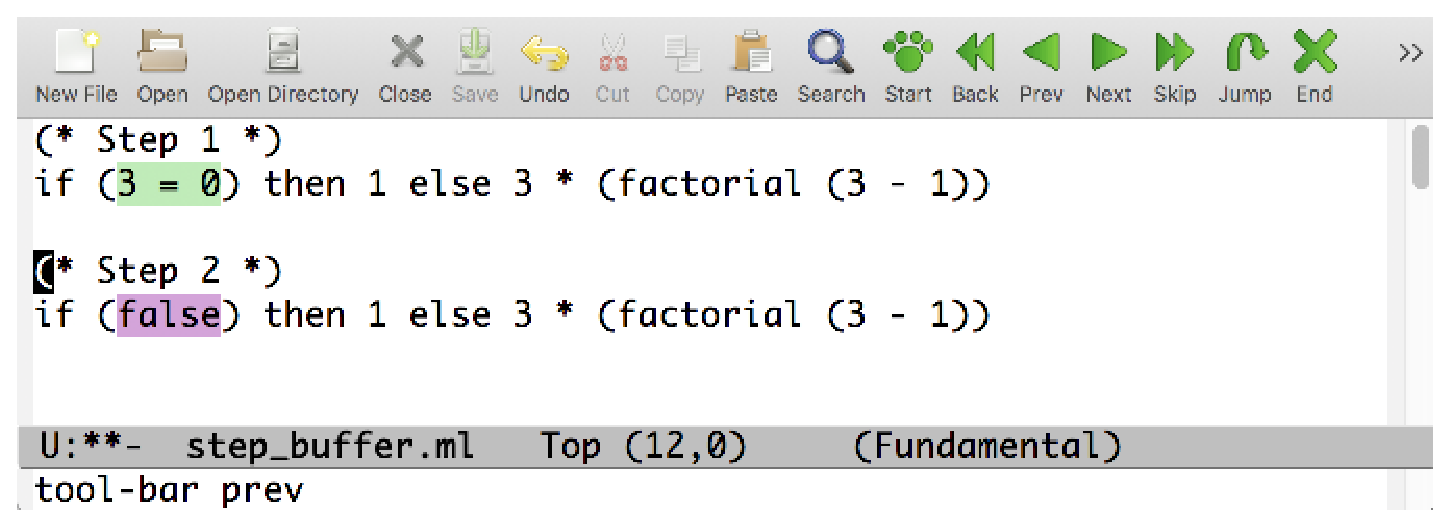
\includegraphics[width=13cm]{1/ocamlfac.eps}
\caption{本研究で実装した OCaml のステッパ}
\label{figure:ocamlfac}
\end{figure}

この中で最も重要なのは 2 つ目、すなわち
入力プログラムを表す構文木を受け取ってステップを表す文字列を出力する関数を作ることである。
この関数は基本的には入力プログラムを実行する関数なので、
インタプリタ関数の一種である。本論文ではこれ以降、この関数のことを「ステッパ関数」と呼ぶ。

インタプリタ関数に出力機能を加えたものがステッパ関数であるが、
プログラムがどのように書き換わっていくかを示すために、
どのステップでも簡約している部分の式だけでなくプログラム全体を出力する必要がある。
そのため、部分式を再帰的に実行する際にその部分式の外の式の情報 (コンテキスト) を
保持する必要がある。

本論文では、まず例外処理の言語機能 try-with に対するステッパ関数を実装した。
その際には、コンテキストを表現できるデータ型を定義し、
それを利用してコンテキストの情報を保持するインタプリタを作ることで
実装することができた。
その実装をもとにして、OCaml の try-with を含む一部の構文のステッパツール
(図 \ref{figure:ocamlfac}) も実装した。

しかし、コンテキストを表現するデータ型は言語ごとに定義しなければならず、
その構造は自明ではない。
そこで次に、継続を明示的に扱うことができる制御オペレータ
algebraic effects (代数的効果) に対するステッパ関数を実装する際には、
インタプリタ関数を機械的にプログラム変換することによって
コンテキストの型とステッパ関数を導出することができた。

そして OCaml ステッパを実際に大学の授業において使用し、
学生のプログラム実行ログやアンケートをもとに評価を行った。
その結果、さまざまな構文の実行においてステッパの需要があったことや、
正しいプログラムを有意に早く書けるようになる場合があったことから、
ステッパの学習的効果を示した。

また、実装した OCaml ステッパは構文解析とステップ実行と表示の
3 つの手順を順番に同期的に行っており、
大規模なプログラムをステップ実行する際に 2 つ目のステップ実行に長い時間がかかるため
表示を始めることができないという問題点があった。
その解決のため、1 ステップの実行と表示処理を交互に行うので
ステップ実行処理の終了を待たずに利用できる「incremental なステッパ」を実装した。

プログラムを 1 ステップずつ実行することは
small-step のインタプリタの動作そのものであるが、
本論文では全体を通して big-step のインタプリタを基にしてステッパ関数を実装する。
その理由は保守性と、
プログラム全体の流れを分かりやすくするためにまとまったステップを省略する機能を
実装するのに必要だからである。

\vspace{1cm}
以下に本論文の構成を示す。{\bf 第2章}では、関連研究について述べる。
{\bf 第3章}では、try-with を含む言語を対象にしたステッパの実装方法を説明する。
{\bf 第4章}では、algebraic effects含む言語を対象にしたステッパ関数のプログラム変換による実装方法を説明する。
{\bf 第5章}では、1 ステップずつ実行する incremental なステッパの実装方法を紹介する。
{\bf 第6章}では、プログラミング学習におけるステッパの効果を考察する。
そして{\bf 第7章}で、結論を述べる。

本論文の第3章と第6章の内容は、我々が2019年に発表した論文 \cite{FCA19} を
もとに発展させた■■ものである。

\pagenumbering{arabic}

\chapter{関連研究}
\label{chapter:related}

\section{ステッパの実装}
\label{section:stepper__related}

ステッパはもともと Racket 言語の教育用に制限された構文に対して作られた。
これは Clements ら \cite{clements01} が設計したもので、
スタックに continuation mark と呼ばれるマークをつけることで
現在の評価文脈を再構成できるようにしている。
この Racket のステッパの対象構文には例外処理が含まれていない。

Whitington と Ridge \cite{EPTCS294.3} は
small-step のインタプリタを直接書くことで
OCaml に対するステッパを実装した。

PLT Redex \cite{felleisen09}は操作的意味論の形式化のための言語で、
文法と簡約規則を定義できるようになっており、DrRacket のステッパを継承している。
さらに、一画面の中に各ステップでのプログラムを配置し、
あるプログラムが1ステップ簡約されて別のプログラムになることを矢印で表したグラフを表示する。
これはより視覚的に簡約の様子を表すことができるほか、
各矢印にそのステップの簡約規則が添えられているのでよりステップを辿りやすい。
しかし、複数のステップのプログラムが同じ画面に表示されている上に
簡約が起こる部分式が強調されていないので、
長いプログラムをステップ実行すると見づらくなってしまう。

根岸ら\cite{NI2009}の関数型言語 Haskell のデバッガフロントエンドは、
一般的なデバッガの実行方法が通用しない遅延評価型言語の
グラフィカルなユーザインタフェースでのステップ実行を含むデバッガ操作を可能にした。
デバッガがブラウザ上で利用できるようになっており、
DrRacket や本研究のステッパと同様に各ステップでのプログラムを、
評価中の式をハイライトしながら表示する。
実行するファイルや、ブレイクポイントをどの関数に設定するか、
ステップ実行するか次のブレイクポイントまで実行するか、
などといった設定をブラウザ上のボタンなどをクリックすることで行うことができる。
デバッガのインタフェースでの本研究との違いは、
根岸ら\cite{NI2009}のデバッガではブレイクポイントをユーザが簡単に設定できるのに対して、
本研究ではブレイクポイントは自動的に全ての簡約基に設定され、
ユーザは詳細に実行のしかたを決められない代わりに「次のステップ」「前のステップ」
などのボタンを押すのみのより簡単な操作のみでステップ実行をすることができる。

\section{ステップ実行によるプログラミング学習}

Tunnel Wilson et al. \cite{tunnell18} は、
代数学的ステッパの出力のような内容を学生に手書きで書かせることによって、
学生がプログラムの実行のされかたをどのように理解しているか、
どのような構文のステップの書き下しができないかといった傾向を分析した。

\section{algebraic effects}
\label{section:algebraic effects__related}

本論文では algebraic effects に対する意味論を、
big-step で書かれた、ハンドラ内の実行について CPS になっているインタプリタで定義する。
Kammar ら \cite{10.1145/2500365.2500590} は small-step で意味論を与えた。
Hillerstr{\"o}m ら \cite{e6cb0c3222794e48bf38cf44e46fe4aa} は
CPS による意味論を与えたが、入力言語を A-正規形に制限しているのに加え、
継続がフレームのリストで与えられており、通常の CPS インタプリタにはなっていない。

上記以外の algebraic effects に関する研究としては、ハンドラの挙動が異
なる shallow ハンドラの研究 \cite{10.1007/978-3-030-02768-1_22} や
algebraic effects を含むプログラムに関する論理関係を
定義する研究 \cite{10.1145/3158096} などがあげられる。本論文で扱ってい
るハンドラは従来の deep ハンドラである。shallow ハンドラにも対応できると
考えているが、これは今後の課題である。


\chapter{try-with 構文のステップ実行}
\label{chapter:try-with}

\section{はじめに}
\label{section:try-with__intro}

この章では、try-with 構文を含む言語を対象としたステッパ関数を
OCaml で実装する方法を示す。
OCaml 自体も try-with 構文で例外処理を行うので、
実際に我々が大学の授業において使っている OCaml ステッパは本章で説明する方法に基づいて実装されている。
ここでは簡単のため型無し $\lambda$ 計算と try-with 構文のみから成る言語を対象として説明する。

ステッパの実装は対象言語の通常のインタプリタ関数を拡張することによって行う。
この章ではまず \ref{section:try-with__interpreter} 節で言語とそのインタプリタを定義し、
\ref{section:try-with__stepper} 節でインタプリタを拡張してステッパを実装する。


 \section{対象言語とインタプリタの定義}
\label{section:try-with__interpreter}

\begin{figure}
\begin{spacing}{0.8}
\begin{verbatim}
type e_t = Var of string               (* x *)
         | Fun of string * e_t         (* fun x -> e *)
         | App of e_t * e_t            (* e e *)
         | Try of e_t * string * e_t   (* try e with x -> e *)
         | Raise of e_t                (* raise e *)
\end{verbatim}
\end{spacing}
\caption{Syntax}
\label{figure:typee}
\end{figure}

\begin{figure}
\begin{spacing}{0.8}
\begin{verbatim}
(* 入力プログラムの例外の値を持った例が *)
exception Error of e_t

(* 式を実行する *)
(* eval : e_t -> e_t *)
let rec eval expr = match expr with
  | Var (x) -> failwith ("unbound variable: " ^ x)  (* ここには来ない *)
  | Fun (x, e) -> Fun (x, e)
  | App (e1, e2) ->
    begin
      let v2 = eval e2 in
      let v1 = eval e1 in
      match v1 with
      | Fun (x, e) ->
        let e' = subst e x v2 in   (* e[v2/x] *)
        let v = eval e' in
        v
      | _ -> failwith "not a function"
    end
  | Try (e1, x, e2) ->
    begin
      try
        let v1 = eval e1 in
        v1
      with Error (v) ->
        let e2' = subst e2 x v in   (* e2[v/x] *)
        eval e2'
    end
  | Raise (e) ->
    let v = eval e in
    raise (Error (v))

(* 実行を開始する *)
(* start : e_t -> e_t *)
let start e =
  try
    eval e
  with
    Error v -> Raise v
\end{verbatim}
\end{spacing}
\caption{Big-step interpreter}
\label{figure:interpreter}
\end{figure}


%In Figures \ref{figure:typee} and \ref{figure:interpreter},
%we define the object language as well as a big-step interpreter.
%The \texttt{eval} function evaluates a given expression following OCaml's call-by-value, right-to-left strategy.
型無し$\lambda$計算と try-with から成る言語の OCaml による定義を
図 \ref{figure:typee} に示す。
そしてこの言語に対する call-by-value かつ right-to-left のインタプリタは図 \ref{figure:interpreter} のように定義できる。
%For instance, when given an application \texttt{e1 e2},
%it first evaluates the argument \texttt{e2}, then evaluates the function \texttt{e1}.
%Once the application has been turned into a redex, we perform $\beta$-reduction, and evaluate the post-reduction expression.
例えば関数適用 \texttt{e1 e2} を実行するときには、
まず引数部分 \texttt{e2} を実行して、次に関数部分 \texttt{e1} を実行する。
両方が値になったら $\beta$ 簡約を行い、簡約後の式を実行する。
%Note that, when the top-level expression is an executable, closed program, the input of the \texttt{eval} function cannot be a variable.  The reason is that we never touch a function's body before it receives an argument, and that $\beta$-reduction replaces lambda-bound variables with values.
引数 \texttt{expr} が変数 \texttt{Var} だった場合はエラー終了するように書かれているが、
これは入力されたプログラム全体が実行可能な閉じた式だった場合に
関数 \texttt{eval} の引数に変数がくることはありえないからである。
なぜありえないかというと、関数の本体の実行は必ず、引数を受け取って仮引数を実引数に置き換えた後に行うからである。

%Object-level exception handling is performed by the meta-level \texttt{try} and \texttt{raise} constructs.
入力プログラムの例外処理は、インタプリタで実際に(OCaml の機能の) \texttt{try} と \texttt{raise} を使って実行する。
%Specifically, when evaluating \texttt{raise e},
%we first evaluate \texttt{e} to some value \texttt{v},
%and then raise a meta-level (OCaml) exception \texttt{Error v}.
具体的には、式 \texttt{raise e} を実行する場合、
まず \texttt{e} を実行してその値 \texttt{v} を得る。
そしてメタレベルの (OCaml の) 例外 \texttt{Error v} を起こす。

%If an exception \texttt{Error v} was raised
%during evaluation of \texttt{e1} in \texttt{try e1 with x -> e2},
%the \texttt{eval} function ignores the rest of the computation in \texttt{e1},
%and evaluates \texttt{e2} with \texttt{v} substituted for \texttt{x}.
式 \texttt{try e1 with x -> e2} の \texttt{e1} を実行している間に
例外 \texttt{Error v} が発生した場合は、
関数 \texttt{eval} は \texttt{e1} の中の残りの計算を無視して、
\texttt{e2} の中の変数 \texttt{x} に値 \texttt{v} を代入した
式 \texttt{e2[v/x]} の実行に移る。
% This is exactly how OCaml's try-with construct works.
このように、OCaml の try-with 構文を利用して OCaml の try-with 構文と同じような動作を実現することができる。
%For convenience, we will hereafter call \texttt{e1} a \emph{tryee};
%the intention is that \texttt{e1} is
%the expression being ``tried'' by the handler.
説明を簡単にするため、 \texttt{try e1 with x -> e2} の \texttt{e1} のことを
以後 \emph{tryee} と呼ぶ。
これは、 try ハンドラによって「try されている」ということを意図している。


%The main function \texttt{start} calls \texttt{eval}
%in an exception handling context.
メイン関数である \texttt{start} が \texttt{eval} を呼び出すとき、
その呼び出しは try-with で囲まれている。
%From the construction,
%we can see that any expression that has a \texttt{raise e}
%with no matching \texttt{try} clause will be evaluated to \texttt{raise v}.
\texttt{Error v -> raise v} とあるように、
対応する \texttt{try} 節が無い \texttt{raise e} の実行結果は、
\texttt{e} の実行結果を \texttt{v} として \texttt{raise v} とする。
%For example, \texttt{2 + 3 + (raise 4) + 5} evaluates to \texttt{raise 4}.
例えば、 \texttt{2 + 3 + (raise 4) + 5} の実行結果は \texttt{raise 4} である。


\section{ステッパの実装}
\label{section:try-with__stepper}

% As stated in Section \ref{sec:intro},
% a stepper must display the whole program at each reduction step.
ステッパは各簡約ステップでのプログラムの全体を表示する必要がある。
% Consider the simple arithmetic expression \texttt{(1 + 2 * 3) + 4}.
% When step-executing this expression,
% we want to see the following reduction sequence:
例えば単純な算術式 \texttt{(1 + 2 * 3) + 4} をステップ実行するとき、
我々が期待するステップ列は以下である。
\[
\begin{array}{cl}
            & \mathtt{(1 + 2 * 3) + 4} \\
\rightarrow & \mathtt{(1 + 6) + 4} \\
\rightarrow & \mathtt{7 + 4} \\
\rightarrow & \mathtt{11}
\end{array}
\]

% The interpreter in Figure \ref{figure:interpreter}, however,
% does not immediately give us these steps.
しかし、図\ref{figure:interpreter} のプログラムに出力機能を加えても、
直ちにこのようなステップ出力は得られない。
% Suppose the \texttt{eval} function is evaluating
% the subexpression \texttt{2 * 3}.
関数 \texttt{eval} が部分式 \texttt{2 * 3} を実行している時のことを考えてみよう。
% We can display this subexpression using a printing function,
% but we do not have enough information to reconstruct the whole program.
式を出力する関数を用意すれば実行中の部分式 \texttt{2 * 3} は表示できるが、
プログラム全体を再構成するには情報が足りていない。
% What is missing here is the \emph{context} surrounding \texttt{2 * 3},
% namely \texttt{(1 + [.])\ + 4}
% (where \texttt{[.]} denotes the hole of the context).
ここで欠けているのは \texttt{2 * 3} を囲んでいる \emph{コンテキスト} すなわち
\texttt{(1 + [.])\ + 4} である。
(コンテキストの穴を \texttt{[.]} と表記する。)
% Hence, to implement a stepper,
% we need to keep track of every evaluation context we have traversed.  
したがって、ステッパを実装するためには、
それまでの評価文脈を追い続ける必要がある。

% In Figure \ref{figure:simpleplug},
% we define context frames as algebraic data of type \texttt{frame\_t}.
図 \ref{figure:simpleplug} で、 \texttt{frame\_t} 型の代数的データとしてコンテキストフレームを定義している。
% Each frame represents evaluation of some subexpression:
各フレームがなんらかの部分式の実行を表しており、
% \eg, \texttt{CAppR (e1)} tells us that we are evaluating
% the argument part of an application, whose function part is \texttt{e1}.
例えば \texttt{CAppR (e1)} は、関数部分が \texttt{e1} である関数適用の引数部分を
実行していることを表す。
% Evaluation contexts are defined as lists of these frames
% (spoiler alert: this does not work for exceptions).
評価文脈はこのフレームのリストで定義される。
% We then define the \texttt{plug} function,
% which reconstructs a program by wrapping the expression
% \texttt{expr} with context frames in \texttt{ctxt}. 
また■■、式 \texttt{expr} をコンテキストフレーム列 \texttt{ctxt} で囲んで
プログラムを再構成する関数 \texttt{plug} も定義する。

\begin{figure}
\begin{spacing}{0.8}
\begin{verbatim}
(* コンテキストフレーム *)
type frame_t = 
             | CAppR of e_t           (* e [.] *)
             | CAppL of e_t           (* [.] v  *)
             | CTry of string * e_t   (* try [.] with x -> e *)
             | CRaise                 (* raise [.] *)

(* コンテキスト *)
type c_t = frame_t list

(* 式全体を再構成する *)
(* plug : e_t -> c_t -> e_t *)
let rec plug expr ctxt = match ctxt with
  | [] -> expr
  | CAppR (e1) :: rest -> plug (App (e1, expr)) rest
  | CAppL (e2) :: rest -> plug (App (expr, e2)) rest
  | CTry (x, e2) :: rest -> plug (Try (expr, x, e2)) rest
  | CRaise :: rest -> plug (Raise expr) rest
\end{verbatim}
\end{spacing}
%\caption{Contexts and reconstruction function; first attempt}
\caption{コンテキストと再構成関数 (試作版)}
\label{figure:simpleplug}
\end{figure}

% Now, if we let the evaluation function receive
% an additional argument representing the context,
% we should be able to display all the steps of
% the arithmetic expression \texttt{(1 + 2 * 3) + 4}.
これで■■、関数 \texttt{eval} がコンテキストを表す追加の引数を受け取るようにすれば、
\texttt{(1 + 2 * 3) + 4} のような式のステップ表示ができるようになるはずである。
% For instance, when evaluating the subexpression \texttt{2 * 3},
% the extra argument will be a two-element list
% \texttt{[(1 + [.]);\ ([.]\ + 4)]},
% and we can obtain the whole program using the \texttt{plug} function.
例えば、部分式 \texttt{2 * 3} を実行している時、その新しい引数の値は
\texttt{[(1 + [.]);\ ([.]\ + 4)]} であり、
これを関数 \texttt{plug} に渡せばプログラム全体を得ることができる。

% The resulting stepper is essentially the CK abstract machine
% \cite{FF1986}, where the expression is the control string and the
% evaluation context is the continuation.
最終的に得られるステッパ■■は、式を control string■■、評価文脈を継続とみなすと、本質的にCK 機械 \cite{FF1986} であるといえる。
% Substitution is used to implement $\beta$-reduction.
% 代入は $\beta$ 簡約の実装のために用いられている■■。
% We did not implement the abstract machine directly but augmented a
% big-step interpreter, because we want to keep the correspondence between
% big-step execution and small-step execution.
big-step インタプリタと small-step インタプリタの実行の対応を維持するため、
抽象機械を直接実装するのではなく big-step インタプリタの拡張によって実装した。
% 抽象マシンを直接実装するのではなく、
% 大きなステップの実行と小さなステップの実行との対応を維持したいため、
% 大きなステップのインタープリターを追加しました。
% It enables us to skip evaluation of user-specified function application,
% as we elaborate in Section~\ref{sec:imp:ocaml}.
big-step インタプリタを基にすることで、ユーザが指定した関数適用をスキップすることができる
(\ref{subsection:skip} 節で触れる)。

% Unfortunately,
% this na\"ive implementation does not work
% in the presence of exception handlers.
しかし、この実装は例外処理について正しく機能しない。
% Consider \texttt{try (2 + 3 * (raise 4) + 5) with x -> x}.
例えば、 \texttt{try (2 + 3 * (raise 4) + 5) with x -> x} について考える。
% When step-executing this expression, we expect to see the following steps:
この式をステップ実行する時、我々が期待するステップは以下である。

\vspace{0.2cm}

\noindent \texttt{(* Step 0 *) try (\colorbox{lightgreen}{2 + (3 * (raise 4)) + 5}) with x -> x\\
  (* Step 1 *) try (\colorbox{purple}{raise 4}) with x -> x\\
  (* Step 1 *) \colorbox{lightgreen}{try (raise 4) with x -> x}\\
  (* Step 2 *) \colorbox{purple}{4}\\
}

\vspace{0.2cm}

% \noindent The first reduction happens when the input
% to the stepping interpreter is \texttt{raise 4}.
\noindent 最初の簡約はステッパ関数に \texttt{raise 4} が渡されたときに起こる。
% However, observe that the highlighted redex is a bigger expression
% \texttt{(2 + 3 * (raise 4) + 5)},
% because reduction of a \texttt{raise} construct discards
% the context \emph{within} the tryee.
しかし、最初のステップでハイライトされている式はそれよりも大きい式
\texttt{(2 + 3 * (raise 4) + 5)} である。
これは \texttt{raise 4} の実行で例外を起こす際に、この式の外側にある、tryee の内部のコンテキストを捨てるからである。
% Since context frames are collected in a single list,
% the second argument at this point will be
% \texttt{[(3 * [.]); (2 + [.]);\ ([.]\ + 5);\ (try [.]\ with x -> x)]},
% \ie, it contains the context \emph{outside} the tryee.
コンレキストフレームは 1 つのリストに入っているので、この時点での関数 \texttt{eval} の第2引数は
\texttt{[(3 * [.]); (2 + [.]);\ ([.]\ + 5);\ (try [.]\ with x -> x)]} であり、
すなわち tryee の外側のコンテキストを含んでいる。
% This suggests that, when dealing with exception handlers,
% we have to distinguish between contexts inside and outside a tryee.
例外処理を扱う場合には、tryee の内側と外側のコンテキストを区別する必要があるということである。
\footnote{
% The destination is not necessary,
% if we want to support only exception handling.
例外処理をサポートするだけならばこの■■必要はない。
% We could simply search for the enclosing handler in the evaluation
% context.
コンテキストフレームのリストを単純に検索すれば最も内側のハンドラを見つけることができるからである。
% However, it requires a linear search through the evaluation context.
しかし、それには評価文脈を線形探索する必要がある。
% Furthermore, distinction is necessary if we want to implement
% more general control operators,
% such as shift and reset \cite{DF1990}.
さらに、shift/reset のようなより一般的な制御オペレータ■■を実装する場合には
この区別が必要になる。
}

\begin{figure}
\begin{spacing}{0.8}
\begin{verbatim}
(* コンテキストフレーム *)
type frame_t = 
             | CAppR of e_t          (* e [.] *)
             | CAppL of e_t          (* [.] v *)
             | CRaise                (* raise [.] *)

(* try フレーム *)
type ctry_t = 
            | CHole                        (* [.] *)
            | CTry of string * e_t * c_t   (* try [.] with x -> e *)

(* コンテキスト *)
and c_t = frame_t list * ctry_t

(* tryee を再構成する *)
(* plug_in_try : e_t -> frame_t list -> e_t *)
let rec plug_in_try expr ctxt = match ctxt with
  | [] -> expr
  | first :: rest -> match first with
    | CAppR (e1) -> plug_in_try (App (e1, expr)) rest
    | CAppL (e2) -> plug_in_try (App (expr, e2)) rest
    | CRaise -> plug_in_try (Raise (expr)) rest

(* プログラム全体を再構成する *)
(* plug : e_t -> c_t -> e_t *)
let rec plug expr (clist, tries) =
  let tryee = plug_in_try expr clist in
  match tries with
  | CHole -> tryee
  | CTry (x, e2, outer) -> plug (Try (tryee, x, e2)) outer
\end{verbatim}
\end{spacing}
%   \caption{Contexts and reconstruction function; final version}
  \caption{コンテキストと再構成関数 (最終版)}
  \label{figure:typec}
\end{figure}

% In Figure \ref{figure:typec},
% we present a refined definition of evaluation contexts.
図 \ref{figure:typec} に、改良したコンテキスト定義を示す。
% We see a new definition of context frames \texttt{frame\_t},
% where \texttt{CTry} is missing.
新しい \texttt{frame\_t} 型の定義は、 \texttt{CTry} を含まないようになっている。
% When evaluating a program that uses try-with constructs,
% these frames are used to build a delimited context within a tryee.
\texttt{frame\_t} 型のフレームは、try-with 構文を使うプログラムを実行において
tryee の内部に限定されたコンテキストを表すために使う。
% We next find a separate datatype \texttt{ctry\_t},
% which can be understood as meta contexts.
次に、別の型 \texttt{ctry\_t} が定義されており、これはメタコンテキストを表す型である。
% Then we define evaluation contexts as pairs of delimited and meta contexts.
そしてコンテキストは tryee 内部に限定されたコンテキストとメタコンテキストの 2 つ組として定義される。
% As an example, when evaluating \texttt{raise 4} in the following expression:
例として、以下のプログラムの中の \texttt{raise 4} を実行しているとき、

\begin{verbatim}
0 + (try 1 + 2 * (try (3 + raise 4) - 5 with x -> x + 6) with y -> y)
\end{verbatim}
% \noindent the current context looks like:
\noindent 現在のコンテキストは以下のようになっている。
\begin{verbatim}
([(3 + [.]); ([.] - 5)],
  CTry ("x", x + 6,
    ([2 * [.]; 1 + [.]],
      CTry ("y", y,
        ([0 + [.]], CHole)))))
\end{verbatim}

% The refined contexts allow us to first reconstruct the expression up to
% the tryee using the \texttt{frame\_t} contexts,
% and then build up the whole program using the \texttt{ctry\_t} contexts.
このようにコンテキスト定義を改良すると、
まず \texttt{frame\_t} 型のコンテキストを使って tryee 式を再構成し、
その後 \texttt{ctry\_t} 型のコンテキストを使ってプログラム全体を作ることができる。
% In our particular example, the stepper reconstructs \texttt{(3 + raise 4) - 5},
% highlights it, and reconstructs the whole program.
上の例でいうと、ステッパはまず \texttt{(3 + raise 4) - 5} を再構成して
ハイライトしてから、プログラム全体を再構成している。

% To give the reader a better idea how context frames are accumulated,
% let us demonstrate the evaluation of an expression involving exception handling:
コンテキストフレームが蓄積されていく様子を具体的に紹介するため、
例外処理を含んだ式の実行で関数 \texttt{eval} がどのような順で再帰呼び出しされるかを以下に示す。

\begin{verbatim}
eval (2 * (try 3 + (raise 4) - 5 with x -> x + 6)) ([], CHole)
eval (try 3 + (raise 4) - 5 with x -> x + 6) ([2 * [.]], CHole)
eval (3 + (raise 4) - 5) ([], CTry ("x", x + 6, ([2 * [.]], CHole)))
eval 5 ([3 + (raise 4) - [.]], CTry ("x", x + 6, ([2 * [.]], CHole)))
eval (3 + (raise 4)) ([[.] - 5], CTry ("x", x + 6, ([2 * [.]], CHole)))
eval (raise 4) ([3 + [.]; [.] - 5], CTry ("x", x + 6, ([2 * [.]], CHole)))
eval 4 ([raise [.]; 3 + [.]; [.] - 5], CTry ("x", x + 6, ([2 * [.]], CHole)))
eval (4 + 6) ([2 * [.]], CHole)
\end{verbatim}

% \noindent Observe that we discard the context within the tryee,
% namely \texttt{3 + (raise [.])\ - 5}, at the last step.
\noindent 最後のステップにおいて、tryee の内部のコンテキスト
すなわち \texttt{3 + (raise [.])\ - 5} が捨てられている。

% Now we present our stepping interpreter in Figure \ref{figure:stepper}.
以上を踏まえ、ステッパ関数を図 \ref{figure:stepper} および図 \ref{figure:try-with__memo} に示す。
% The function extends the big-step interpreter in two ways
% (as shaded in the figure):
この関数は通常の big-step インタプリタを以下の 2 点において拡張したものである (図中の灰色の部分)。
% (i) it receives an argument representing the evaluation context;
(i) コンテキストを表す引数を受け取るようにする。
% and (ii) it outputs the current program every time reduction takes place.
(ii) 簡約が行われる全ての箇所で簡約前後のプログラムをそれぞれ出力する。

\begin{figure}
%(* add a non-try frame *)
%(* add : c_t -> frame_t -> c_t *)
%let rec add (list, outer) ctxt = (ctxt :: list, outer)
%
%(* add a try frame *)
%(* add_try : c_t -> string -> e_t -> c_t *)
%let rec add_try ctxt var expr = ([], CTry (var, expr, ctxt))  
\begin{spacing}{0.8}
\begin{alltt}
(* ステッパ関数 *)
(* eval : e_t -> c_t -> e_t *)
let rec eval expr \colorbox{lightgray}{ctxt} = match expr with    (* コンテキストのための引数を増やす *)
  | Var (x) -> failwith ("unbound variable: " ^ x)
  | Lam (x, e) -> Lam (x, e)
  | App (e1, e2) ->
    begin
      let v2 = eval e2 \colorbox{lightgray}{(add ctxt (CAppR e1))} in     (* コンテキスト情報を足す *)
      let v1 = eval e1 \colorbox{lightgray}{(add ctxt (CAppL v2))} in     (* コンテキスト情報を足す *)
      match v1 with
      | Lam (x, e) ->
        let e' = subst e x v2 in
        \colorbox{lightgray}{memo (App (v1, v2)) e' ctxt;}                                (* 出力 *)
        let v = eval e' \colorbox{lightgray}{ctxt} in                     (* コンテキスト情報を足す *)
        v
      | _ -> failwith "not a function"
    end
  | Try (e1, x, e2) ->
    begin
      try
        let v1 = eval e1 \colorbox{lightgray}{(add_try ctxt x e2)} in     (* コンテキスト情報を足す *)
        \colorbox{lightgray}{memo (Try (v1, x, e2)) v1 ctxt;}                             (* 出力 *)
        v1
      with Error (v) ->
        let e2' = subst e2 x v in
        \colorbox{lightgray}{memo (Try (Raise v, x, e2)) e2' ctxt;}                       (* 出力 *)
        eval e2' \colorbox{lightgray}{ctxt}                               (* コンテキスト情報を足す *)
    end
  | Raise (e0) ->
    let v = eval e0 \colorbox{lightgray}{(add ctxt CRaise)} in            (* コンテキスト情報を足す *)
    \colorbox{lightgray}{begin match ctxt with                   }
\end{alltt}
\vspace{-27pt}
\begin{alltt}
    \colorbox{lightgray}{    | ([], _) -> ()                     }
\end{alltt}
\vspace{-27pt}
\begin{alltt}
    \colorbox{lightgray}{    | (clist, tries) ->                 }
\end{alltt}
\vspace{-27pt}
\begin{alltt}
    \colorbox{lightgray}{      memo (plug_in_try (Raise v) clist)}                        (* 出力 *)
\end{alltt}
\vspace{-27pt}
\begin{alltt}
    \colorbox{lightgray}{           (Raise v)                    }
\end{alltt}
\vspace{-27pt}
\begin{alltt}
    \colorbox{lightgray}{           ([], tries)                  }
\end{alltt}
\vspace{-27pt}
\begin{alltt}
    \colorbox{lightgray}{end;                                    }
    raise (Error (v))
\end{alltt}
\end{spacing}
% \caption{Stepping evaluator}
\caption{ステッパ関数}
\label{figure:stepper}
\end{figure}

\begin{figure}
\begin{spacing}{0.8}
\begin{alltt}
(* 簡約前の式と簡約後の式とコンテキストを受け取ってステップを出力する *)
(* memo : e_t -> e_t -> c_t -> unit *)
let memo expr1 expr2 ctxt =
  print_exp (plug (green expr1) ctxt);
  print_exp (plug (purple expr2) ctxt)

(* ステップ実行を始める *)
(* start : e_t -> e_t *)
let start e =
  try
    eval e \colorbox{lightgray}{([], CHole)}    (* 空のコンテキスト *)
  with
    Error (v) -> (Raise v)
\end{alltt}
\end{spacing}
% \caption{\texttt{memo} and main functions}
\caption{関数 \texttt{memo} とメイン関数}
\label{figure:try-with__memo}
\end{figure}

% Let us observe the application case.
まず関数適用 \texttt{e1 e2} のケースの動作を見ると、以下のようになっている。
% As in the big-step interpreter,
% we first evaluate \texttt{e2}, and then \texttt{e1}.
通常のインタプリタと同じように、最初に \texttt{e2} を実行してその後に \texttt{e1} を実行する。
% When \texttt{e1} has reduced to a function,
% we know that the application is a $\beta$-redex.
\texttt{e1} の実行結果が関数であれば、関数適用式は $\beta$ 簡約基になっている。
% In the standard interpreter,
% what we do is to perform the substitution \texttt{subst e x v2}
% and then evaluate the result.
通常のインタプリタでは、そこで代入 \texttt{subst e x v2} をしてその結果を実行する。
% In the stepper, on the other hand,
% we have an additional function call to the \texttt{memo} function
% defined in Figure \ref{figure:memo}.
それに対しステッパでは、
図 \ref{figure:try-with__memo} で定義された関数 \texttt{memo} の呼び出しが追加されている。
% This function receives three arguments:
% the redex we have just found, its reduct, and the current evaluation context.
この関数は 3 つの引数を受け取る。
見つかった簡約基と、その簡約結果と、現時点のコンテキストである。
% When given these arguments,
% the \texttt{memo} function reconstructs and prints the pre- and post-reduction programs,
% using the \texttt{plug} and \texttt{print\_exp} functions
関数 \texttt{memo} はこれらの引数を受け取ったら、
関数 \texttt{plug} と \texttt{print\_exp} を使って簡約前と後のプログラムをそれぞれ再構成して出力する。
\footnote{
    % In the actual implementation,
    % we annotate redexes and reducts using OCaml's \emph{attributes}.
    実際の実装においては、簡約基と簡約後の式の範囲を表す情報をつけるのに
    OCaml の \emph{attributes} という機能を利用している。
    % Here, we write \texttt{green expr1} to mean \texttt{expr1[@stepper.redex]},
    % and similarly for \texttt{purple}.
    ここでは \texttt{green expr1} は \texttt{expr1[@stepper.redex]} と出力される式を表し、
    \texttt{purple} についても同様である。
    % When displaying the steps,
    % the Emacs Lisp program uses the attributes information
    % to appropriately highlight expressions.
    ステップを表示する際に、 Emacs Lisp のプログラムがその情報から
    適切に式をハイライトする。
    }
    % .  After printing the programs, we continue evaluation as usual.
    。プログラムを出力したら、普通の実行を再開する。

% In the \texttt{eval} function, we find three more occurrences of \texttt{memo},
% representing the following reduction rules:
関数 \texttt{eval} では、これ以外にあと 3 箇所で関数 \texttt{memo} が呼び出されている。
それらはそれぞれ以下の簡約規則を表している。

\begin{itemize}
  \item \texttt{try v with x -> e} $\leadsto$ \texttt{v}
  \item \texttt{try raise v with x -> e2} $\leadsto$ \texttt{subst e2 x v}
  \item \texttt{...\ (raise v) ...} $\leadsto$ \texttt{raise v}
\end{itemize}

% \noindent Note that,
% although the second reduction always happens right after the third one,
% we keep them as separate rules.
\noindent 2 つ目の簡約は必ず 3 つ目の簡約の直後に起こるが、
それにもかかわらずこれらを別の規則として扱っていることに注目してほしい。
% The reason is that we need the latter to reduce
% a raise construct with no matching try clause:
その理由は、例えば \texttt{3 + (raise 4) - 5} $\leadsto$ \texttt{raise 4} のように
対応する try 節が無い \texttt{raise} 式の簡約に 3 つ目の規則が必要だからである。
% \eg, \texttt{3 + (raise 4) - 5} $\leadsto$ \texttt{raise 4}.
% Separating the two reductions also has an educational benefit:
% it clearly tells us that exception handling consists of two tasks:
% discarding the context and substituting the value.
また、これらの規則を別にしておくのは教育上の意義もある。
それは、例外処理が「コンテキストを捨てること」と「例外の値を代入すること」
の 2 つの動作で成り立っていることが明確にステップに表れることである。

%% By observing what we pass to the \texttt{memo} function, we can see the reduction rules of the object language.  In the definition of \texttt{eval}, we have four occurrences \texttt{memo}, representing the following reduction rules:

%% \begin{enumerate}
%% \item
%%   \texttt{(fun x -> e) v} $\leadsto$ \texttt{subst e x v}
%%   \begin{itemize}
%%   \item \texttt{\colorbox{lightgreen}{f 4} + 100} (where \texttt{f = fun x -> x * 2 + 1}) reduces to \texttt{(\colorbox{purple}{4 * 2 + 1}) + 100}.
%%   \end{itemize}
%% \item
%%   \texttt{try v with x -> e} $\leadsto$ \texttt{v}
%%   \begin{itemize}
%%   \item \texttt{\colorbox{lightgreen}{try 2 with x -> x * x}} reduces to \texttt{\colorbox{purple}{2}}.
%%   \end{itemize}
%% \item
%%   \texttt{try raise v with x -> e2} $\leadsto$ \texttt{subst e2 x v}
%%   \begin{itemize}
%%   \item \texttt{\colorbox{lightgreen}{try raise 4 with x -> x * x}} reduces to \texttt{\colorbox{purple}{4 * 4}}.
%%   \end{itemize}
%% \item
%%   \texttt{try ...\ (raise v) ...\ with x -> e2} $\leadsto$ \texttt{try raise v with x -> e2}
%%   \begin{itemize}
%%   \item \texttt{try \colorbox{lightgreen}{1 + 2 + (raise 4) - 5} with x -> x * x} reduces to \texttt{try \colorbox{purple}{raise 4} with x -> x * x}.
%%   \end{itemize}
%% \end{enumerate}


\section{おわりに}
\label{section:try-with__conclusion}

この章では、例外処理の構文 try-with に対応したステッパを、
インタプリタを拡張することによって実装する方法を示した。

まず、 try-with 構文に対する通常の big-step インタプリタは
実際の OCaml の try-with を用いて実装することができた。

ステッパへの拡張においては、各ステップでのプログラム全体を表示するために、
実行中の部分式のコンテキストの情報が必要である。
例外発生によって一度に捨てられる範囲のコンテキスト、
すなわち try 節の内側のコンテキストフレームのリストをひとまとめにして、
そのリストのような構造としてコンテキストを定義した。
それをインタプリタの再帰の構造にしたがって要素を足しながら引数に渡すようにすると
実行中の部分式のコンテキストの情報が得られるようになり、
プログラム全体が出力できるステッパが得られた。



\chapter{algebraic effects のステップ実行}
\label{chapter:algebraic effects}

\section{はじめに}
\label{section:algebraic effects__intro}

プログラムのある時点での残りの計算のことを「継続」という。
たとえばプログラム \texttt{1 + (2 + 4)} の \texttt{2 + 4} を計算している時点での
継続は「今の計算の結果を \texttt{1} に足す」という計算である。
継続のうち一部を切り取った計算を限定継続という。
\ref{chapter:try-with} 章で扱った例外処理機能 try-with は、
「例外が起きたらその時点での継続のうち try までの限定継続を捨てる」
ものだといえる。
一方、shift/reset \cite{DF1990} や algebraic effects \cite{PRETNAR201519}
といった言語機能では、継続を関数のようなものとして変数に束縛し、
値に適用することができる。
このような機能を含むプログラムの制御の移り変わりは複雑なので、
これを対象にしたステッパ関数の実装は try-with の場合よりも困難である。

\ref{chapter:try-with} 章で示したステッパ関数の実装方法では、
プログラム出力に必要なコンテキスト情報の構造を自分で定義し、
インタプリタに追加して引数で適切にフレームを足していく必要があった。
単純な言語に対するステッパであれば、手動でコンテキストの型を定義するのは簡単だが、
言語が複雑になってくると必ずしもこれは自明ではない。
実際、 \ref{chapter:try-with} 章でのコンテキストは try-with 構文で区切る必要があったため
構造が一次元的でなく、リストのリストになった。
algebraic effects などが入った場合、どのようなコンテキストを使えば良いのかは別途、
考慮する必要がある。
そこで、本研究ではインタプリタを機械的にプログラム変換することで
ステッパおよび必要なコンテキストの構造を導出した。
本章では algebraic effects を含む言語についてこの導出の過程を説明する。

まず \ref{section:definition} 節で algebraic effects を含む言語およびそのインタプリタを定義し、
\ref{section:transform} 節でインタプリタを変換してステッパを得る過程を説明する。
\ref{section:languages} 節では他のいくつかの言語に対するステッパ関数を
同様の変換によって得ることについて議論し、
\ref{section:conclusion} 節でまとめる。

またこの章でのもう1つの貢献として、
algebraic effects の big-step インタプリタを定義した (\ref{subsection:1cps} 節)。
これは、 \ref{chapter:try-with} 章でのステッパ実装と同様に
big-step のインタプリタを元にしてステッパ関数を作成するというアプローチをとったため、
元のインタプリタが必要になったからである。


\input{4/definition}

\input{4/transform}

\input{4/languages}

\section{この章のまとめ}
\label{section:conclusion}

ステッパ関数を実装するためには、
コンテキストの情報を保持しながら部分式を再帰的に実行するインタプリタを作ればよい。
\ref{chapter:try-with} 章で行った方法では言語ごとにコンテキストを表すデータ型を
考えた上でインタプリタに実行の流れに従った新しい引数を付け足す作業が必要だったが、
本研究では通常のインタプリタをCPS変換および非関数化するという機械的な操作で
コンテキストの型およびコンテキストの情報を保持するインタプリタ関数を導出した。

その方法で、継続を明示的に扱える algebraic effects を含む言語に対するステッパ関数を実装し、
他の例外処理機能である try-with や shift/reset を含む言語についても同様の変換ができることを確認した。



\chapter{5}
\label{chapter:experiment}

\section{Stepping OCaml in the Classroom}
\label{sec:exp}
Since 2016, we have been using (earlier versions of) our stepper in an
introductory OCaml course called ``Functional Programming'',
taught by the third author at Ochanomizu University.

\subsection{The OCaml Course}
The ``Functional Programming'' course teaches how to program with functions and types, covering
basic topics such as recursion, datatypes, effects, and modules.
The course consists of 15, weekly lab sessions, and each session
 consists of 90 minutes lab-style class per week.
(Many students remain in the lab after 90 minutes up until around 150
minutes.)
Throughout the course, students build a program that searches for
the shortest path based on Dijkstra's algorithm.
The participants of the course are second-year undergraduate students
majoring in computer science (around 40 students each year).
All students enter this course after a CS 1 course in the C
programming language.

The course is taught in a ``flipped classroom'' style.
Before every meeting, students are asked to study assigned readings
and videos prepared by the instructor and answer simple quizzes.
In the classroom, they practice the newly covered topics
through exercises, with assistance of the instructor as well as five
to six teaching assistants (including the first and second authors).  

The exercises include simple practice problems and report problems.
The former are for confirming students' understanding of the
topics and are expected to be completed within a class.
The latter problems (for credit) are due in one week.
Whenever a student executes a program, by either step execution or
standard execution, the program as well as its execution log (syntax
errors, type errors, or the result of execution) are recorded.

For most of the problems (up to the 12th week), we provide a check system
where students can submit their solutions to see whether they pass the
given tests.
To earn points for report problems, students are required to have their
programs pass the check system.

\subsection{The Uses of the Stepper}
We introduced the stepper into Functional Programming in 2016.
Although the steppers used in the past had almost the same user-interface as the one shown in Figure \ref{figure:ocamlfac}, they differ in the following ways:
\begin{description}
\item[2016] This first version supported function definitions,
conditionals, records, lists, and recursion.  However, there were
various operations that were not supported.
As such, the usability of the stepper was low.
Moreover, when the instructor introduced the stepper to students, he
only mildly encouraged to use it.
Although we do not know how much the stepper was used in 2016 since we
did not log the execution of stepper, we expect it was used
only rarely in the first few weeks of the course.
\item[2017] Based on the lessons from the previous year, the second
version supported most operations used in the first six weeks.
The instructor introduced the stepper up front at the first class and
showed how to use the stepper with various examples in the subsequent
classes.
\item[2018] The third version supported almost all the constructs
needed for the course, including modules, exception handling,
sequential execution, printing, references, and arrays.
It also supported skipping of function application.
The instructor introduced the stepper as though the stepper was the
only way to execute OCaml programs, encouraging the uses of the
stepper.
(Students gradually realized that they could execute a program in the
interpreter in a few weeks.)
\end{description}

\begin{figure}
  \begin{center}
    \includegraphics[width=15cm]{6/table1a.eps}
    \caption{Frequency of standard execution (light-colored) and step execution (dark-colored) in each week in 2017 and 2018. The stepper was not used at all toward the end of the course in 2017, but it was used in some degree in 2018.}
    \label{figure:allExecution}
  \end{center}
\end{figure}

\begin{figure}[!t]
  \begin{center}
    \includegraphics[width=15cm]{6/table1b.eps}
    \caption{Number of times the stepper was used to evaluate a program with ``try'', ``module'', ``print'' or ``ref'' in 2018.}
    \label{figure:stepExecution}
  \end{center}
\end{figure}

Figure \ref{figure:allExecution} shows how many times students used the stepper among all the executions including the ones that ended up in an error.
%% Table~\ref{TableUsage} shows how many times students used the stepper
%% (the column ``step.'') among all the executions (``all'') including the
%% ones that ended up in an error.
%% The table further shows a breakdown of the step-executed programs.
In both 2017 and 2018, the stepper was used quite often until week 5.
This is partly because
we encouraged students to use the stepper when they had
trouble finding bugs and understanding recursion.
After week 5, the number decreases, because students started using an
interpreter, too, as programs became larger.

In 2017, the number of stepper uses decreases toward the end of the
course.
In contrast, in 2018, certain number of stepper uses is observed,
thanks to the support of exception handling, modules, and references.
Figure \ref{figure:stepExecution} shows the number of execution of programs using these features during step-execution in 2018. % 足した execution を単数にした
From the figure, we can see that there is a demand for step
%% From the table, we observe that some students try to see step
execution of advanced constructs such as exception handling and
modules.

The exact numbers of execution are available in Table \ref{TableUsage} in the Appendix.
%% These graphs were generated from Table \ref{TableUsage} of the Appendix.

\subsection{Effects of Stepper}
It is not easy to see the effect of a tool like a stepper on
the learning of students.
In the case of improving error messages of a compiler, for example,
one can classify various errors and see how many of them are covered
by the improved error messages objectively.
For the stepper, it is unclear how to show such numeric data.

\begin{figure}
  \begin{center}
    \includegraphics[width=15cm]{6/table2.eps}
    \caption{Number of questions where students arrived at a correct answer significantly faster in 2017 and 2018 than 2016.}
    \label{figure:p}
  \end{center}
\end{figure}

As an attempt to measure the effect of the stepper, we examined how
long students took to submit correct solutions to the check system.
Among all the submitted correct solutions, we gathered the (wall-clock) times of
submissions recorded in the check system that are within 100 minutes
from the beginning of the class and compared the average times among
2016, 2017, and 2018.
%% Table~\ref{TableTTest} shows the result.

Figure \ref{figure:p} shows the number of questions for which students submitted a correct answer within significantly shorter time in 2017 and 2018 compared to 2016.  The data are based on one-sided t-testing with p-value $< 0.05$; we refer the reader to Table \ref{TableTTest} of the appendix for details.
Note that we did not include week 1 because we had a special pre-test in the first lecture in 2018.
%% For all the problems from week 2 to week 12 (the last week where the
%% check system is available), the average time of correct submissions in
%% 2018 is compared to that of 2016 and 2017.
%% We did not include week 1, because we had a special pre-test in the
%% first lecture in 2018.
%% The problem numbers that start with ‘r’ are for practice problems, which are mostly solved in the day of the lecture. The ones without are report problems, some of which are difficult and are solved only later in the week.
%% The figure shows how many questions students submitted correct answers in 2017 or 2018 significantly earlier than in 2016 for each lecture, based on one-sided t-testing with p-value $<0.05$ (Detailed values are listed in Table \ref{TableUsage} in the appendix) .
%% The table shows the result of one-sided t-testing with p-values,
%% whether the use of the stepper in 2017 and 2018 makes the average time
%% earlier than in 2016.

From the figure, we can see improvement of submission times after the (real) introduction of the stepper, especially in earlier problems.
%% From the figure, we observe that for both 2017 and 2018, the average
%% times of correct solutions for many problems (in particular, the easier
%% ones) are significantly earlier than 2016.
However, there is an exception: for one problem in the 6th week, correct submissions come significantly later in 2018 than in 2016.
%% One exception is for the problem 6.r1 in 2018.
%% For this problem, the average time for 2018 is significantly later
%% than 2016.
The problem simply asks students to write a recursive function that adds 1 to each
element of a given list.
We do not know why it took so long in 2018.
The result of t-testing all the problems together is t(1778) = 2.819 (p=0.002) in 2017 and t(2111) = 2.592 (p=0.005) in 2018.
%% The last row shows the result of t-testing all the problems together,
%% which shows the same trend as most of the problems.
%% This could be partly attributed to the uses of the stepper for better
%% understanding the behavior of programs.

We also compared the average times between 2017 and 2018.
For earlier weeks (up to week 5), submissions in 2017 were
significantly earlier, while for later weeks,
there were no significant difference
(except for two problems where the average
times for 2018 were earlier).
Putting all the problems together, the two were not significantly
different with t(1953)=0.455 (p=0.324).

\paragraph{Threats to validity.}
It is possible that the results of our experiment were affected by the enrolled students in each year (there was no over-lapping).
In all the three years, 
the instructor started the class with some introductory comments that
vary in length.
Although the instructor made similar comments in each year, they were
not exactly the same, which could have affected.

\subsection{Students' Evaluation}

\begin{table}
  \begin{center}
  \begin{tabular}{|l|c|r|}
    \hline
    & score & \# of students \\ \hline
    Using the stepper, I could almost always understand & & \\
    the behavior of programs or the cause of errors. & 4 & 3 \\ \hline
    Using the stepper, I could often solve problems at hand. & 3 & 8\\ \hline
    Using the stepper, I could sometimes solve problems at hand. & 2 & 25\\ \hline
    I could rarely find new things using the stepper. & 1 & 2\\ \hline
    The stepper was useless.  I did not use the stepper. & 0 & 0\\ \hline
%   4 & ステッパを使えばほぼ必ずプログラムの動きや間違いの原因が分かった & 3\\ \hline
%   3 & ステッパを使って問題を解決できることが多くあった & 8\\ \hline
%   2 & たまにステッパを使って問題を解決できることがあった & 25\\ \hline
%   1 & ステッパを使うことで新たに何かが分かることはほとんど無かった & 2\\ \hline
%   0 & 全く役に立たなかった、または使わなかった & 0\\ \hline
  \end{tabular}
  \end{center}
  \caption{Students' scoring of the stepper in 2018.
  38 students out of 42 answered.
  The average is 2.3.}
% 平均 2.3158、38 / 42 人が回答
  \label{TableScore}
\end{table}

At the end of the semester of 2018, we asked the students to share
their thoughts on the stepper.
We received responses from 38 out of 42 students.
We first asked whether the stepper was useful on the 0 to 4 point scale.
The results, which we present in Table \ref{TableScore}, suggest
that the stepper is not a silver bullet that is useful
for all the time.
However, most students could solve the problems at hand sometimes
using the stepper.
We are encouraged to see some students choose ``the stepper was almost always useful''.

We next asked students to write when the stepper was useful (if any),
such as when they found their misunderstanding, or when they could
deepen their understanding.
We summarize the answers in two categories.

\paragraph{Understanding of the behavior of programs.}
Seven students answered they could deepen their understanding of
the behavior of programs.
In particular, five students among them wrote explicitly that the
stepper helped them figure out how functions consume recursive data.
We imagine it was particularly instructive to see how a recursive 
function definition is unfolded in nesting application.
% TODO: この文の意味が不明

Other students answered that they could observe the behavior of
programs in general.
They found that arguments of a function are evaluated before the
function call, and that the elements of a list are evaluated one by one.
Among them, one student observed the right-to-left execution
employed in OCaml.
Previously, such subtle behavior was taught only in passing without
much emphasis.

\paragraph{Debugging.}
Many students found the stepper useful for debugging.
Sixteen students answered they could find what was wrong when their
program did not pass test cases.
By observing each step of execution, they could identify when the
program behaved differently from their expectation.
This is an important step toward debugging in general.
Because printing (and side effects) is handled at the end of the
course, the only debugging method for students had been unit testing:
they checked whether all the component functions worked as expected.
With the stepper, they can simply observe execution of the program and
see when it goes wrong.

Three students found the stepper useful to understand why their
program did not terminate.
Without printing, it is not easy for students to identify the cause of
infinite loops.
Using the stepper, one of the students could not only observe
the infinite loop, but also see how far her program went well
and when it went wrong.



\chapter{評価}
\label{chapter:experiment}

% \section{はじめに}
% \label{section:experiment__intro}
% セクションにする意味なかったか

2016 年度以降、我々は \ref{section:ocaml stepper} で述べた OCaml ステッパを
% Since 2016, we have been using (earlier versions of) our stepper in an
% introductory OCaml course called ``Functional Programming'',
% taught by the third author at Ochanomizu University.
お茶の水女子大学で毎年前期に開講されている授業「関数型言語」において利用してきた。
この章では、授業で実際に学生に OCaml ステッパを使ってもらったことで
得られた実行ログやアンケート結果からステッパの教育的効果について考察する。

まず \ref{section:experiment__course} 節で
ステッパを使用した授業の内容や進め方について説明する。
そして \ref{section:experiment__result} 節でステッパの効果について考察する。


\section{授業の内容}
\label{section:experiment__course}
% The ``Functional Programming'' course teaches
% how to program with functions and types, covering
% basic topics such as recursion, datatypes, effects, and modules.
「関数型言語」は OCaml を用いて関数型プログラミングを学ぶ授業であり、
再帰、データ型、副作用、モジュールなどの基本的な言語機能を扱う。
% The course consists of 15, weekly lab sessions, and each session
%  consists of 90 minutes lab-style class per week.
学期全体を通して、学生はダイクストラ法に基づいて最短路問題を解くプログラムを作成する。
授業は週に1回、90分間で、全15回で構成されている。
% (Many students remain in the lab after 90 minutes up until around 150
% minutes.)
(授業終了後も教室に残って作業を続ける学生も多い。)
% Throughout the course, students build a program that searches for
% the shortest path based on Dijkstra's algorithm.
% The participants of the course are second-year undergraduate students
% majoring in computer science (around 40 students each year).
% All students enter this course after a CS 1 course in the C
% programming language.
受講者は情報科学を専攻する学部2年生で、毎年40人程度である。
全ての学生がこの授業より前にC言語によるプログラミングを経験している。

% The course is taught in a ``flipped classroom'' style.
この授業では「反転授業」を行なっている。
反転授業とは、学生が各自内容を予習し、授業時間は講義を行わず演習などに活用する授業形態である。
% Before every meeting, students are asked to study assigned readings
% and videos prepared by the instructor and answer simple quizzes.
この授業では、学生は毎週の授業の前に、この授業に向けた教科書 \cite{Asai07} と教員が作成した動画による予習をし、
インターネット上で数問の簡単な問題に解答する。
% In the classroom, they practice the newly covered topics
% through exercises, with assistance of the instructor as well as five
% to six teaching assistants (including the first and second authors).  
授業時間内には、学生はその回に新しく取り上げた内容に関する演習問題に取り組み、
教員および5〜8人のティーチングアシスタントに質問することができる。

% The exercises include simple practice problems and report problems.
演習問題はほとんどが要求を満たす関数を実装するというものであり、
「練習問題」と「レポート課題」に分かれている。
% The former are for confirming students' understanding of the
% topics and are expected to be completed within a class.
練習問題は学生がどの程度その回の内容を理解しているか確認するための簡単な問題で、
授業時間内に解くことを期待している。
% The latter problems (for credit) are due in one week.
レポート課題は評定に利用する問題■■で、締め切りが1週間後に設定されている。

授業をする演習室では常に OCaml プログラム実行のログをとっている。
% Whenever a student executes a program, by either step execution or
% standard execution, the program as well as its execution log (syntax
% errors, type errors, or the result of execution) are recorded.
学生がプログラムを実行する時には必ず、ステッパによる実行と通常の実行のどちらも、
プログラム全文と実行ログが記録される。

% For most of the problems (up to the 12th week), we provide a check system
% where students can submit their solutions to see whether they pass the
% given tests.
解答プログラムが合っているかどうかを確認する方法の 1 つとして、
「チェックシステム」を用意してある。
チェックシステムは教員が用意した単体テストに通るかどうかを確認できるプログラムで、
問題ごとに用意されており、12 週目までのほとんどの問題を対象にしている。
各学生が各問題のチェックシステムに初めて通った時には学生の ID が記録されるようになっており、
% To earn points for report problems, students are required to have their
% programs pass the check system.
締め切りまでに 1 度以上チェックシステムに通ることが、レポート課題の各問で点を得る条件に含まれている。


\section{結果}
\label{section:experiment__result}

ステッパの学習的効果を評価するため、我々は以下の項目について調査した。

\begin{itemize}
\item ステッパがどれほど使われていたか
\item ステッパをよく使った年と使わなかった年で学生の解答の速さに違いがあったか
\item 学生がステッパについてどう感じたか
\end{itemize}

ステッパがどれほど使われたかについては、 OCaml 実行ログからステッパによる実行とそうでない実行の数を数えた。
解答の速さの差は、チェックシステムに記録されている時刻、
すなわち学生が初めて正解のプログラムをチェックシステムに通した時刻から統計的に分析した。
最後の項目については、学生にアンケートを取った。

% \subsection{The Uses of the Stepper}
\subsection{ステッパの使用状況}
\label{subsection:result__uses}

% We introduced the stepper into Functional Programming in 2016.
我々が授業「関数型言語」にステッパを導入したのは 2016 年度である。
% Although the steppers used in the past had
% almost the same user-interface as the one shown
% in Figure \ref{figure:ocamlfac}, they differ in the following ways:
当時のステッパは図 \ref{figure:ocamlfac} とほとんど同じインタフェースだったが、
以下の点で \ref{section:experiment__stepper} 節で紹介したステッパと異なる。
\begin{description}
% \item[2016] This first version supported function definitions,
% conditionals, records, lists, and recursion.  However, there were
% various operations that were not supported.
% As such, the usability of the stepper was low.
\item[2016年度] 最初の OCaml ステッパは
関数定義、条件分岐、レコード、リスト、再帰のような
より基本的な式しか実行できず、使いにくかった。
% Moreover, when the instructor introduced the stepper to students, he
% only mildly encouraged to use it.
また、教員がステッパを学生に紹介する際に、ステッパの使用を強くは奨励しなかった。
% Although we do not know how much the stepper was used in 2016 since we
% did not log the execution of stepper, we expect it was used
% only rarely in the first few weeks of the course.
2016 年度はステッパによるプログラム実行のログを採取していなかったため
ステッパがどれくらい利用されていたのかは不明であるが、
最初の数週にわずかに利用されたのみだと我々は考えている。
% \item[2017] Based on the lessons from the previous year, the second
% version supported most operations used in the first six weeks.
\item[2017年度] 6 週目までに学習する構文要素のほとんどに対応したステッパを利用した。
% The instructor introduced the stepper up front at the first class and
% showed how to use the stepper with various examples in the subsequent
% classes.
教員は最初の授業で事前にステッパを紹介し、
その後の授業でも様々な例でステッパを利用して見せた。
% \item[2018] The third version supported almost all the constructs
% needed for the course, including modules, exception handling,
% sequential execution, printing, references, and arrays.
\item[2018年度] \ref{section:experiment__stepper} 節で紹介した、
モジュール、例外処理、逐次実行、配列などを実行できるステッパを利用した。
これは授業範囲のほとんどの構文要素を含んでいる。
% It also supported skipping of function application.
また関数適用のスキップ機能も追加した。
% The instructor introduced the stepper as though the stepper was the
% only way to execute OCaml programs, encouraging the uses of the
% stepper.
教員は、まるでステッパでしかプログラムが実行できないかのように学生に紹介することで、
学生にステッパの利用を促した。
% (Students gradually realized that they could execute a program in the
% interpreter in a few weeks.)
(数週の間に学生は普通のインタプリタで実行ができることにだんだん気付いていった。)
\end{description}

\begin{figure}
  \begin{center}
    \includegraphics[width=15cm]{6/table1a.eps}
    % \caption{Frequency of standard execution (light-colored) and
    % step execution (dark-colored) in each week in 2017 and 2018.
    % The stepper was not used at all toward the end of the course in 2017,
    % but it was used in some degree in 2018.}
    \caption[ステッパが使用された回数]{
        2017年度と2018年度の各週の、通常の実行 (薄い色) とステップ実行 (濃い色) の回数。
        2017年度は終盤では全く使われなくなったが、2018年度にはある程度使われ続けている。
    }
    \label{figure:allExecution}
  \end{center}
\end{figure}

\begin{figure}[!t]
  \begin{center}
    \includegraphics[width=15cm]{6/table1b.eps}
    % \caption{Number of times the stepper was used to evaluate
    % a program with ``try'', ``module'', ``print'' or ``ref'' in 2018.}
    \caption[ステッパの実行のうち各構文を含むプログラムの実行の回数]{
        try、module、print、ref を含むプログラムのステッパによる実行の回数
    }
    \label{figure:stepExecution}
  \end{center}
\end{figure}

% Figure \ref{figure:allExecution} shows
% how many times students used the stepper
% among all the executions including the ones that ended up in an error.
図 \ref{figure:allExecution} は、
全受講生の全実行 (エラー終了した実行を含む) のうち何回がステッパでの実行だったかを示すグラフである。
% In both 2017 and 2018, the stepper was used quite often until week 5.
2017 年度と 2018 年度の両方で、5 週目まではステッパが頻繁に利用されている。
% This is partly because
% we encouraged students to use the stepper when they had
% trouble finding bugs and understanding recursion.
この一因は、バグの発見や再帰の理解のためにステッパを使うように
教員やティーチングアシスタントが学生に勧めたことである。
% After week 5, the number decreases, because students started using an
% interpreter, too, as programs became larger.
6週目以降は、学生がインタプリタに気付き始めたことと
実行するプログラムが大きくなったことにより使用回数が減少した。

% In 2017, the number of stepper uses decreases toward the end of the
% course.
2017 年度には、ステッパの使用回数は最後の授業に近づくにつれて減少している。
% In contrast, in 2018, certain number of stepper uses is observed,
% thanks to the support of exception handling, modules, and references.
それに対して 2018 年度は、例外処理、モジュール、逐次実行、書き換え可能な変数に対応したので、
ある程度の回数の使用が見られる。
% Figure \ref{figure:stepExecution} shows the number of execution of
% programs using these features during step-execution in 2018. % 足した execution を単数にした
図 \ref{figure:stepExecution} は、2018 年度のステップ実行のうち
この年に新しく対応した構文を利用したプログラムの実行の回数のグラフである。
% From the figure, we can see that there is a demand for step
% execution of advanced constructs such as exception handling and
% modules.
どの構文もいくらかステップ実行されており、
例外処理やモジュールのような高度な構文のステップ実行の需要があることが分かる。

% The exact numbers of execution are available in Table \ref{TableUsage} in the Appendix.
図 \ref{figure:allExecution} と図 \ref{figure:stepExecution}
のグラフの正確な数値は付録の表 \ref{TableUsage} に掲載する。

% \subsection{Effects of Stepper}
\subsection{ステッパの効果}
\label{subsection:result__effects}

% It is not easy to see the effect of a tool like a stepper on
% the learning of students.
ステッパのようなツールの教育効果を測ることは簡単ではない。
% In the case of improving error messages of a compiler, for example,
% one can classify various errors and see how many of them are covered
% by the improved error messages objectively.
例えばコンパイラのエラーメッセージ改善の評価ならば、
エラーを分類して改善されたエラーメッセージがそのうちどれほどに対応しているかを見ることができるだろう。
% For the stepper, it is unclear how to show such numeric data.
ステッパにおいては、そういった定量的なデータをどのように示せばよいかが不明瞭である。

\begin{figure}
  \begin{center}
    \includegraphics[width=15cm]{6/table2.eps}
    % \caption{Number of questions where students arrived
    % at a correct answer significantly faster in 2017 and 2018 than 2016.}
    \caption[学生が正答するまでの時間の比較]{
        2017年度と2018年度に、学生が2016年度より有意に早く正答を提出した問題の数
    }
    \label{figure:p}
  \end{center}
\end{figure}

% As an attempt to measure the effect of the stepper, we examined how
% long students took to submit correct solutions to the check system.
ステッパの効果を測定するための試みとして、
我々は学生がチェックシステムに正しい解答を提出するまでにかかった時間を調査した。
% Among all the submitted correct solutions, we gathered the (wall-clock) times of
% submissions recorded in the check system that are within 100 minutes
% from the beginning of the class and compared the average times among
% 2016, 2017, and 2018.
全ての問題のチェックシステムに記録されている「正答が初めて提出された時刻」の中から
授業開始から100分以内の時刻を収集し、2016年、2017年、2018年の間で比較した。

% Figure \ref{figure:p} shows the number of questions
% for which students submitted a correct answer
% within significantly shorter time in 2017 and 2018 compared to 2016.
図 \ref{figure:p} は
2017 年度と 2018 年度それぞれの、2016 年度よりも
学生が有意に短い時間で正解を提出した問題の数を示している。
% The data are based on one-sided t-testing with p-value $< 0.05$;
% we refer the reader to Table \ref{TableTTest} of the appendix for details.
このデータは p $< 0.05$ の片側 t 検定に基づいており、
詳しい数値は付録の表 \ref{TableTTest} にある。
% Note that we did not include week 1
% because we had a special pre-test in the first lecture in 2018.
ただし、2018 年度のみ初回の授業に特別なテストを行ったので、
第 1 週はこの調査の対象から外した。

% From the figure, we can see improvement of submission times
% after the (real) introduction of the stepper, especially in earlier problems.
図から、実質的なステッパの導入の後、提出までの時間が改善されていることが分かる。
序盤の問題で特に改善が見られる。
% However, there is an exception: for one problem in the 6th week,
% correct submissions come significantly later in 2018 than in 2016.
しかし 1 つ例外があり、第 6 週の 1 つの問題のみ、
2018 年度の正解提出が有意に 2016 年度よりも遅かった。
% The problem simply asks students
% to write a recursive function that adds 1 to each
% element of a given list.
該当する問題は、リストを受け取ったらそのリストの全要素に 1 を足したリストを返す
再帰関数を書くという単純な問題である。
% We do not know why it took so long in 2018.
この問題の正答が 2018 年度に遅くなった理由は分からない。
% The result of t-testing all the problems together is
% t(1778) = 2.819 (p=0.002) in 2017 and t(2111) = 2.592 (p=0.005) in 2018.
全問題の正答時間をまとめて t 検定した結果は、2017 年度が t(1778) = 2.819 (p=0.002)、
2018 年度が t(2111) = 2.592 (p=0.005) だった。

% We also compared the average times between 2017 and 2018.
2017 年度と 2018 年度の平均時間も比較した。
% For earlier weeks (up to week 5), submissions in 2017 were
% significantly earlier, while for later weeks,
% there were no significant difference
% (except for two problems where the average
% times for 2018 were earlier).
第 5 週までの早い週には 2017 年度の方が有意に早く、
それより後は 2 問のみ 2018 年度の方が早く、あとは有意差は見られなかった。
% Putting all the problems together, the two were not significantly
% different with t(1953)=0.455 (p=0.324).
こちらも全問題の時間をまとめて t 検定すると、t(1953)=0.455 (p=0.324) となり、
有意な差はなかった。

% \paragraph{Threats to validity.}
\paragraph{有効性に対する脅威}
% It is possible that the results of our experiment were affected
% by the enrolled students in each year (there was no over-lapping).
この調査の結果は、各年の学生の影響を受けた可能性がある (同じ学生が 2 度以上履修したことはない)。
% 実験の結果は、毎年入学した学生の影響を受けた可能性があります(重複はありませんでした)。
% In all the three years, 
% the instructor started the class with some introductory comments that
% vary in length.
また、3 年間を通して
毎回の授業時間の最初に教員が前回の課題や今回の内容などについて話す時間をとっており、
その長さは毎回同じではなかった。
% Although the instructor made similar comments in each year, they were
% not exactly the same, which could have affected.
毎年ほとんど同じようなコメントをしてはいるが完全に同じではないので、結果に影響した可能性がある。

% \subsection{Students' Evaluation}
\subsection{学生による評価}
\label{subsection:result__students}

\begin{table}
  \begin{center}
  \begin{tabular}{|l|c|r|}
    \hline
    % & score & \# of students \\ \hline
    & 点数 & 人数 \\ \hline
    % Using the stepper, I could almost always understand & & \\
    % the behavior of programs or the cause of errors. & 4 & 3 \\ \hline
    % Using the stepper, I could often solve problems at hand. & 3 & 8\\ \hline
    % Using the stepper, I could sometimes solve problems at hand. & 2 & 25\\ \hline
    % I could rarely find new things using the stepper. & 1 & 2\\ \hline
    % The stepper was useless.  I did not use the stepper. & 0 & 0\\ \hline
    ステッパを使えばほぼ必ずプログラムの動きや間違いの原因が分かった & 4 & 3\\ \hline
    ステッパを使って問題を解決できることが多くあった & 3 & 8\\ \hline
    たまにステッパを使って問題を解決できることがあった & 2 & 25\\ \hline
    ステッパを使うことで新たに何かが分かることはほとんど無かった & 1 & 2\\ \hline
    全く役に立たなかった、または使わなかった & 0 & 0\\ \hline
%   4 & ステッパを使えばほぼ必ずプログラムの動きや間違いの原因が分かった & 3\\ \hline
%   3 & ステッパを使って問題を解決できることが多くあった & 8\\ \hline
%   2 & たまにステッパを使って問題を解決できることがあった & 25\\ \hline
%   1 & ステッパを使うことで新たに何かが分かることはほとんど無かった & 2\\ \hline
%   0 & 全く役に立たなかった、または使わなかった & 0\\ \hline
  \end{tabular}
  \end{center}
%   \caption{Students' scoring of the stepper in 2018.
%   38 students out of 42 answered.
%   The average is 2.3.}
\caption[学生による点数評価]{2018 年度の学生による点数評価。42 人中 38 人が回答。平均は 2.3 だった。}
% 平均 2.3158、38 / 42 人が回答
  \label{TableScore}
\end{table}

% At the end of the semester of 2018, we asked the students to share
% their thoughts on the stepper.
2018 年度前期の最後に、学生にステッパについてのアンケートを実施した。
% We received responses from 38 out of 42 students.
42 人の受講者のうち 38 人が回答した。
% We first asked whether the stepper was useful on the 0 to 4 point scale.
その中で、ステッパがどれくらい便利だったかを 0 から 4 点で評価してもらった。
% The results, which we present in Table \ref{TableScore}, suggest
% that the stepper is not a silver bullet that is useful
% for all the time.
結果を表 \ref{TableScore} に示す。
この表からはステッパはいつでも役立つ万能なツールではないことが分かる。
% However, most students could solve the problems at hand sometimes
% using the stepper.
しかし、多くの学生がステッパを使って時々問題を解決することができている。
% We are encouraged to see some students choose ``the stepper was almost always useful''.
「ステッパを使えばほぼ必ずプログラムの動きや間違いの原因が分かった」を選んだ学生もいた。

% We next asked students to write when the stepper was useful (if any),
% such as when they found their misunderstanding, or when they could
% deepen their understanding.
他の質問で、
プログラムの間違いの発見や理解のためにステッパを活用できた場面を (あれば) 答えてもらった。
% We summarize the answers in two categories.
その答えを 2 つに分類して紹介する。

% \paragraph{Understanding of the behavior of programs.}
\paragraph{プログラムの挙動の理解}
% Seven students answered they could deepen their understanding of
% the behavior of programs.
7 人の学生が、プログラムの挙動についての理解を深めることができたと答えた。
% In particular, five students among them wrote explicitly that the
% stepper helped them figure out how functions consume recursive data.
特にその内 5 人が関数がどのように再帰的なデータを消費するのかを把握するのに役立ったと書いている。
% 特に、そのうち5人の学生は、関数が再帰データをどのように消費するかを把握するのにステッパーが役立つと明示的に書いています。
% We imagine it was particularly instructive to see how a recursive 
% function definition is unfolded in nesting application.
再帰関数定義が展開されて関数適用の入れ子になっていく様子を見ることができることは
再帰の理解の助けになると考えられる。

% Other students answered that they could observe the behavior of
% programs in general.
他の学生は、プログラム全般の動きを観察できたと答えた。
% They found that arguments of a function are evaluated before the
% function call, and that the elements of a list are evaluated one by one.
その学生たちは、引数が関数呼び出しの前に 1 つずつ実行されることを発見した。
% Among them, one student observed the right-to-left execution
% employed in OCaml.
1 人は OCaml プログラムが right-to-left で実行されていることに気付いた。
% Previously, such subtle behavior was taught only in passing without
% much emphasis.
以前は、このような細かい動作について特に強調せず授業を進めていた。

% \paragraph{Debugging.}
\paragraph{デバッグ}
% Many students found the stepper useful for debugging.
多くの学生がデバッグにステッパを利用できたと回答した。
% Sixteen students answered they could find what was wrong when their
% program did not pass test cases.
16 人の学生が、テストを通らなかった時にどこが間違っているのかを見つけることができたと回答した。
% By observing each step of execution, they could identify when the
% program behaved differently from their expectation.
実行の各ステップを観察することで、期待と違った振る舞いをする箇所を特定することができたという。
% This is an important step toward debugging in general.
これは一般的なデバッグをする上で重要な過程である。
% Because printing (and side effects) is handled at the end of the
% course, the only debugging method for students had been unit testing:
% they checked whether all the component functions worked as expected.
この授業では出力などの副作用を終盤で学習するので、
学生のデバッグの方法は単体テストで関数全体が正しい値を返すかどうかを見るしかなかった。
% With the stepper, they can simply observe execution of the program and
% see when it goes wrong.
しかしステッパがあれば、
学生は実行中のどこで間違いが起きているのかを単純に観察することができる。

% Three students found the stepper useful to understand why their
% program did not terminate.
% Without printing, it is not easy for students to identify the cause of
% infinite loops.
また、3 人の学生がプログラムが停止しない時にその原因をステッパで突き止めることができた。
出力機能を使わずに無限ループの原因を特定することにもステッパは利用できる。
% Using the stepper, one of the students could not only observe
% the infinite loop, but also see how far her progr went well
% and when it went wrong.
% ここは書かない・・・



\cite{FCA19}

\newpage
\chapter*{謝辞}

・浅井先生
・叢さん
・石尾氏
・北川氏
・1学年上の研究室の人
・家族
・祖父母
・PPL 2018 と PPL 2019 でなにか言ってくれた人々
・戸次先生
・ステッパを使わされた学生
・株式会社 HERP の人々
〜に感謝いたします.


\newpage
% \input{bibliography}

% ppl2020/0107 から持ってきた
\bibliographystyle{jplain}
\bibliography{stepper}

\newpage

%付録
\appendix
\appendix
\chapter{学生の実行ログから得られたデータ}

\begin{table}[h]
\begin{center}
  \begin{tabular}{|c||c|c|c|c|c|c||c|c|c|c|c|c||l|}
    \hline
    & \multicolumn{6}{|c||}{2017} & \multicolumn{6}{|c||}{2018} & \\ \cline{2-13}
    \hspace{-1mm}week\hspace{-1mm} & all & step. & try & \hspace{-1mm}mod.\hspace{-1mm} & \hspace{-1mm}print\hspace{-1mm} & ref
    & all & step. & try & \hspace{-1mm}mod.\hspace{-1mm} & \hspace{-1mm}print\hspace{-1mm} & ref & contents\\ \hline
    1 & 1293 & 504 & 0 & 0 & 0 & 0 & 1233 & 627 & 0 & 0 & 0 & 0 & fun.\ def.\\ \hline
    2 & 1511 & 235 & 0 & 0 & 0 & 0 & 1375 & 189 & 0 & 0 & 0 & 0 & if\\ \hline
    3 & 1618 & 144 & 0 & 0 & 0 & 0 & 1641 & 179 & 0 & 0 & 0 & 0 & record\\ \hline
    4 & 2364 & 169 & 0 & 0 & 0 & 0 & 2517 & 332 & 0 & 0 & 0 & 0 & list\\ \hline
    5 & 2556 & 193 & 0 & 0 & 0 & 0 & 3173 & 213 & 0 & 0 & 0 & 0 & list 2\\ \hline
    6 & 1596 & 43 & 0 & 0 & 0 & 0 & 1369 & 41 & 0 & 0 & 0 & 0 & Dijkstra\\ \hline
    7 & 2621 & 92 & 0 & 0 & 0 & 0 & 3570 & 86 & 0 & 0 & 0 & 0 & map\\ \hline
    8 & 1874 & 81 & 0 & 0 & 0 & 0 & 2028 & 75 & 0 & 0 & 0 & 0 & filter\\ \hline
    9 & 2184 & 34 & 0 & 0 & 0 & 0 & 3300 & 98 & 0 & 0 & 0 & 0 & gen.\ rec.\\ \hline
    10 & 2254 & 48 & 0 & 0 & 0 & 0 & 3298 & 106 & 3 & 0 & 0 & 0 & tree\\ \hline
    11 & 1783 & 20 & 10 & 0 & 0 & 0 & 2790 & 37 & 22 & 0 & 0 & 0 & exception\\ \hline
    12 & 1785 & 12 & 8 & 4 & 0 & 0 & 3501 & 37 & 3 & 26 & 3 & 0 & module\\ \hline
    13 & 1678 & 10 & 0 & 7 & 2 & 0 & 2943 & 22 & 0 & 3 & 16 & 0 & seq.\ exec.\\ \hline
    14 & 1280 & 11 & 0 & 0 & 0 & 1 & 1511 & 65 & 0 & 4 & 0 & 56 & ref\\ \hline
    15 & 517 & 6 & 0 & 0 & 0 & 0 & 1717 & 68 & 0 & 5 & 0 & 30 & heap\\ \hline
  \end{tabular}
\end{center}
  % \caption{Number of uses of the stepper (step.) among all the
  % executions (all) in 2017 and 2018.  The columns try, mod., print,
  % and ref represent number of uses of the stepper for programs that
  % contain exception handling, modules, printing (and sequential
  % execution), and references (including arrays), respectively.
  % The rightmost column shows representative handled in the
  % week.}
  \caption[ステッパが使用された回数]{
    2017年度と2018年度の全ての実行 (all) のうちステッパの使用回数 (step.)。
    try、mod.、print、ref の列はそれぞれ例外処理、モジュール、標準出力 (と逐次実行)、
    書き換え可能な変数 (配列を含む) を表している。
    右端の列はその週に取り上げた内容である。
  }
  \label{TableUsage}
\end{table}

\begin{table}
\begin{center}  
\small
  \begin{tabular}{|l||c|c|c||c|c|c||l|}
    \hline
    week.
    & \multicolumn{3}{|c||}{2016 to 2017}
    & \multicolumn{3}{|c||}{2016 to 2018}
    &
    \\ \cline{2-7}
    problem & t & p & +/- & t & p & +/- & contents
    \\ \hline
    2.r1
    & t(55)=2.098 & p=\textcolor{red}{0.020} & dec
    & t(60)=0.635 & p=0.264 & dec
    & if\\ \cline{1-7}
    2.r2
    & t(56)=2.364 & p=\textcolor{red}{0.011} & dec
    & t(57)=1.831 & p=\textcolor{red}{0.036} & dec
    & \\ \cline{1-7}
    2.r3
    & t(54)=1.896 & p=\textcolor{red}{0.032} & dec
    & t(59)=0.751 & p=0.228 & dec
    & \\ \cline{1-7}
    2.1
    & t(66)=3.006 & p=\textcolor{red}{0.002} & dec
    & t(74)=3.372 & p=\textcolor{red}{0.001} & dec
    & \\ \cline{1-7}
    2.2
    & t(56)=3.672 & p=\textcolor{red}{0.000} & dec
    & t(62)=3.036 & p=\textcolor{red}{0.002} & dec
    & \\ \hline
    3.r1
    & t(52)=3.222 & p=\textcolor{red}{0.001} & dec
    & t(61)=2.936 & p=\textcolor{red}{0.002} & dec
    & record\\ \cline{1-7}
    3.r2
    & t(42)=2.339 & p=\textcolor{red}{0.012} & dec
    & t(56)=3.467 & p=\textcolor{red}{0.001} & dec
    & \\ \cline{1-7}
    3.r3
    & t(41)=1.373 & p=0.089 & dec
    & t(51)=2.688 & p=\textcolor{red}{0.005} & dec
    & \\ \cline{1-7}
    3.1
    & t(28)=5.610 & p=\textcolor{red}{0.000} & dec
    & t(38)=2.753 & p=\textcolor{red}{0.004} & dec
    & \\ \cline{1-7}
    3.2
    & t(17)=1.655 & p=0.058 & dec
    & t(27)=0.105 & p=0.459 & dec
    & \\ \cline{1-7}
    3.3
    & t(16)=1.546 & p=0.071 & dec
    & t(13)=0.603 & p=0.279 & dec
    & \\ \hline
    4.r1
    & t(47)=2.088 & p=\textcolor{red}{0.021} & dec
    & t(61)=2.446 & p=\textcolor{red}{0.009} & dec
    & list\\ \cline{1-7}
    4.r2
    & t(48)=1.909 & p=\textcolor{red}{0.031} & dec
    & t(60)=2.267 & p=\textcolor{red}{0.014} & dec
    & \\ \cline{1-7}
    4.1
    & t(51)=2.134 & p=\textcolor{red}{0.019} & dec
    & t(60)=2.473 & p=\textcolor{red}{0.008} & dec
    & \\ \cline{1-7}
    4.2
    & t(18)=3.033 & p=\textcolor{red}{0.004} & dec
    & t(20)=0.489 & p=0.315 & dec
    & \\ \hline
    5.r1
    & t(42)=1.037 & p=0.153 & dec
    & t(55)=0.257 & p=0.399 & inc
    & list 2\\ \cline{1-7}
    5.1
    & t(49)=1.592 & p=0.059 & dec
    & t(61)=0.904 & p=0.185 & dec
    & \\ \cline{1-7}
    5.2
    & t(55)=4.138 & p=\textcolor{red}{0.000} & dec
    & t(62)=1.631 & p=0.054 & dec
    & \\ \cline{1-7}
    5.3
    & t(47)=3.305 & p=\textcolor{red}{0.001} & dec
    & t(50)=1.940 & p=\textcolor{red}{0.029} & dec
    & \\ \hline
    6.r1
    & t(30)=0.322 & p=0.375 & inc
    & t(51)=2.011 & p=\textcolor{blue}{0.025} & inc
    & Dijkstra's algorithm\\ \cline{1-7}
    6.1
    & t(41)=1.678 & p=0.050 & dec
    & t(61)=1.155 & p=0.126 & dec
    & \\ \cline{1-7}
    6.2
    & t(45)=1.415 & p=0.082 & dec
    & t(62)=0.976 & p=0.166 & dec
    & \\ \cline{1-7}
    6.3
    & t(34)=2.296 & p=\textcolor{red}{0.014} & dec
    & t(42)=0.548 & p=0.293 & dec
    & \\ \hline
    7.r1
    & t(42)=0.462 & p=0.323 & inc
    & t(56)=0.314 & p=0.377 & dec
    & map\\ \cline{1-7}
    7.r2
    & t(41)=0.286 & p=0.388 & inc
    & t(54)=1.181 & p=0.121 & dec
    & \\ \cline{1-7}
    7.r3
    & t(40)=0.677 & p=0.251 & inc
    & t(51)=1.492 & p=0.071 & dec
    & \\ \cline{1-7}
    7.1
    & t(21)=0.965 & p=0.173 & dec
    & t(20)=0.372 & p=0.357 & dec
    & \\ \cline{1-7}
    7.2
    & t(12)=0.380 & p=0.355 & inc
    & \, t(7)=0.686 & p=0.258 & dec
    & \\ \hline
    8.r1
    & t(46)=1.162 & p=0.126 & inc
    & t(58)=2.694 & p=\textcolor{red}{0.005} & dec
    & filter\\ \cline{1-7}
    8.1
    & t(16)=0.844 & p=0.205 & dec
    & t(22)=0.841 & p=0.205 & dec
    & \\ \hline
    9.r1
    & t(44)=1.294 & p=0.101 & dec
    & t(55)=0.678 & p=0.250 & dec
    & general recursion\\ \hline
    10.r1
    & t(48)=0.312 & p=0.378 & dec
    & t(51)=1.308 & p=0.098 & dec
    & tree\\ \cline{1-7}
    10.r2
    & t(48)=0.457 & p=0.325 & dec
    & t(50)=1.760 & p=\textcolor{red}{0.042} & dec
    & \\ \cline{1-7}
    10.1
    & t(33)=0.976 & p=0.168 & dec
    & t(38)=0.845 & p=0.202 & dec
    & \\ \cline{1-7}
    10.2
    & t(19)=1.498 & p=0.075 & dec
    & t(19)=0.871 & p=0.197 & dec
    & \\ \cline{1-7}
    10.3
    & t(15)=1.538 & p=0.072 & dec
    & t(12)=2.240 & p=\textcolor{red}{0.022} & dec
    & \\ \hline
    11.r1
    & t(43)=0.272 & p=0.393 & dec
    & t(53)=1.555 & p=0.063 & dec
    & exception\\ \cline{1-7}
    11.r2
    & t(37)=0.454 & p=0.326 & dec
    & t(44)=1.906 & p=\textcolor{red}{0.032} & dec
    & \\ \cline{1-7}
    11.r3
    & t(31)=0.050 & p=0.480 & inc
    & t(40)=1.208 & p=0.117 & dec
    & \\ \cline{1-7}
    11.1
    & t(34)=1.567 & p=0.063 & dec
    & t(46)=1.518 & p=0.068 & dec
    & \\ \cline{1-7}
    11.2
    & t(28)=2.204 & p=\textcolor{red}{0.018} & dec
    & t(36)=1.563 & p=0.063 & dec
    & \\ \cline{1-7}
    11.3
    & t(17)=0.604 & p=0.277 & dec
    & t(21)=0.384 & p=0.352 & dec
    & \\ \hline
    12.r1
    & t(39)=2.229 & p=\textcolor{red}{0.016} & dec
    & t(52)=4.009 & p=\textcolor{red}{0.000} & dec
    & module\\ \hline
    all
    & t(1778)=2.819 & p=\textcolor{red}{0.002} & dec
    & t(2111)=2.592 & p=\textcolor{red}{0.005} & dec
    & \\ \hline
  \end{tabular}
  \end{center}
  % \caption{Result of one-sided t-test with p-values comparing
  % the time between the beginning of the class and
  % the moment that students submitted a correct solution.
  % The column +/- shows whether the average time increased or decreased.
  % The p-values below $0.05$ are colored.}
  \caption[拡張されたステッパを利用した年と他の年の学生が正答するまでの時間の比較]{
    授業開始から学生が正解を提出するまでにかかった時間を比較した片側 t 検定の結果と p 値。
    列 +/- は平均値が増加したか減少したかを表している。
    $0.05$ 未満の p 値に色を付けた。
  } 
  \label{TableTTest}
\end{table}


\end{document}
